\documentclass[12pt,a4paper]{article}

\usepackage[dutch]{babel}
\usepackage{listings}

\usepackage[]{algorithm2e}

% Voor todo's
\usepackage{todonotes}

% Voor wiskunde
\usepackage{amsmath}
\usepackage{amsfonts}
\usepackage{amssymb}

% Om het totaal aantal pagina's te tellen
\usepackage{lastpage}

% Voor tekeningen
\usepackage{tikz}
\usetikzlibrary{decorations}
\usetikzlibrary{calc}

% Nog tekeningen
\usepackage{pgfplots}

% Om de marges aan te passen
\usepackage[left=2cm,right=2cm,top=2cm,bottom=2cm]{geometry}

% Voor headers en footers
\usepackage{fancyhdr}
\pagestyle{fancy}

\lhead{Tom Sydney Kerckhove \& Xavier Go\'as Aguililla}
\rhead{\thepage /\pageref{LastPage}}

\lfoot{Practicum}
\cfoot{Toepassingen van Meetkunde in Informatica}
\rfoot{Snijdende Cirkels}

\renewcommand{\headrulewidth}{0.4pt}
\renewcommand{\footrulewidth}{0.4pt}

\begin{document}
\begin{titlepage}
\thispagestyle{empty}
\newcommand{\HRule}{\rule{\linewidth}{0.5mm}}
\center
\textsc{\LARGE KU Leuven}\\[1.5cm]
\vfill

\textsc{\large Practicum}\\[0.5cm]
% \HRule \\[0.4cm]
{ \Huge \bfseries Snijdende cirkels}\\[0.4cm]
% \HRule \\[1.5cm]
\textsc{\large Toepassingen van de meetkunde in de informatica [G0Q37C]}\\[0.5cm]
\vfill

\begin{minipage}{0.4\textwidth}
\begin{flushleft} \large
\emph{Auteurs:}\\
Xavier \textsc{Go\'as Aguililla}\\
Tom Sydney \textsc{Kerckhove}
\end{flushleft}
\end{minipage}
~
\begin{minipage}{0.4\textwidth}
\begin{flushright} \large
\emph{Professor:} \\
prof. dr. ir. Dirk \textsc{Roose}\\
\end{flushright}
\end{minipage}\\[4cm]

{\large \today}\\[3cm]
\vfill

\end{titlepage}
\tableofcontents
\section{Inleiding}
%% \todo{inleiding}


\section{Algoritmen}

\subsection{Snijpunt van twee cirkels berekenen}
\label{sec:snijpunt}

\begin{algorithm}[H]
  \KwData{twee cirkels, C en C' met resp middelpunten $p_{1}, p_{2}$ en stralen $r_{1}, r_{2}$}
  \KwResult{waar als en slechts als de twee cirkels snijden}
  d $\leftarrow$ afstand(p1,p2)\\
  \eIf{($d \leq r_1 + r_2) \land (d \geq abs (r_1 - r_2))$}{
    \Return{true}
  }{
    \Return{false}
  }

 \caption{Nagaan of twee cirkels snijden}
\end{algorithm}

\begin{algorithm}[H]
  \KwData{twee cirkels, C en C' met resp middelpunten $p_{1}, p_{2}$ en stralen $r_{1}, r_{2}$}
  \KwResult{geen, of twee snijpunten van de twee cirkels (die dan identiek zijn)}
  \eIf{$circlesIntersect(c1, c2) \land c1 \neq c2$}{
    px1 $\leftarrow$ s + 2*(y1-y2)/d'*δ\\
    px2 $\leftarrow$ s - 2*(y1-y2)/d'*δ\\
    py1 $\leftarrow$ t - 2*(x1-x2)/d'*δ\\
    py2 $\leftarrow$ t + 2*(x1-x2)/d'*δ\\
    s   $\leftarrow$ ((x1+x2)/2) + (x2-x1)*α\\
    t   $\leftarrow$ ((y1+y2)/2) + (y2-y1)*α\\
    α   $\leftarrow$ (r1*r1-r2*r2)/(2*d')\\
    δ   $\leftarrow$ (1/4) * sqrt ( (d+r1+r2)*(d+r1-r2)*(d-r1+r2)*(r1+r2-d)  )\\
    d'  $\leftarrow$ d*d\\
    d   $\leftarrow$ distance p1 p2\\
    \Return{$\left\{S_1,S_2\right\}$}
  }{
    \Return{$\varnothing$}
  }

 \caption{Snijpunten van twee cirkels berekenen}
\end{algorithm}

\subsection{Na\"ief}
\label{sec:naief}

De naïeve aanpak is gegarandeerd $O(n^2)$ en kunnen we als volgt beschrijven:

\begin{algorithm}[H]
  \KwData{een lijst van $n$ cirkels C, gegeven door hun middelpunt en straal}
  \KwResult{een verzameling van $S$ snijpunten R van de cirkels in C}
  S = $\varnothing$\;
  \For{$i\leftarrow 1$ \KwTo $n$}{
    \For{$j\leftarrow i$ \KwTo $n$}{
      $S = S \cup circleIntersection(c(i),c(j))$
    }

  }
 \caption{Na\"ieve aanpak (imperatief)}
\end{algorithm}

\subsection{Kwadratisch}
\label{sec:kwadratisch}

\subsection{Linearitmisch}
\label{sec:linearitmisch}


\section{Experimenten}
%% \todo{Doubling ratio experiment voor runtime}
%% \todo{experiment ivm stralen}


\begin{figure}[H]
	\centering			
	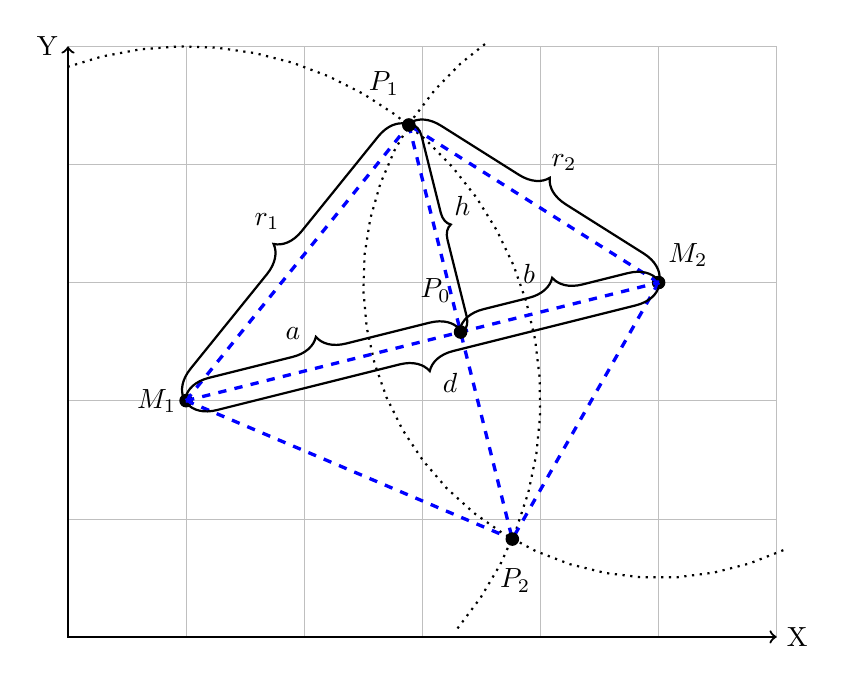
\begin{tikzpicture}[scale=1.5, domain=0:4]
		% grid
      	\draw[very thin,color=lightgray] (0,0) grid (6,5);
      	\draw [<->,thick] (0,5) node (yaxis) [left] {Y} |- (6,0) node (xaxis) [right] {X};

		% Definitions
    	\pgfmathsetlengthmacro{\ra}{3cm}
    	\pgfmathsetlengthmacro{\xa}{1cm}
    	\pgfmathsetlengthmacro{\ya}{2cm}
    
    	\pgfmathsetlengthmacro{\rb}{2.5cm}
    	\pgfmathsetlengthmacro{\xb}{5cm}
    	\pgfmathsetlengthmacro{\yb}{3cm}
	
		% The middlepoints
  		\coordinate (CA) at (\xa,\ya);
  		\coordinate (CB) at (\xb,\yb);
  
  		% The point
  		\draw[fill,color=black] (CA) circle (1.5pt) node[left, color=black] {$M_1$};
  		\draw[fill,color=black] (CB) circle (1.5pt) node[right, yshift=10pt, color=black] {$M_2$};
  
  		% The circle
  		%\draw[dashed,color=black] (CA) circle (\ra);
		%\draw[dashed,color=black] (CB) circle (\rb);
  
		\draw [dotted,thick,domain=-40:110] plot ({1+3*cos(\x)}, {2+3*sin(\x)});
		\draw [dotted,thick,domain=295:125] plot ({5+2.5*cos(\x)}, {3+2.5*sin(\x)});
	
		\coordinate (PA) at (2.885365678957660, 4.333537284169362);
    	\coordinate (PB) at (3.761693144571752, 0.828227421712991);
		\coordinate (PO) at (3.323529411764706, 2.580882352941176);
		
		\draw[very thick,color=blue,dashed] (CA) -- (CB);
      	\draw[very thick,color=blue,dashed] (PA) -- (PB);
      	\draw[very thick,color=blue,dashed] (CA) -- (PA);
      	\draw[very thick,color=blue,dashed] (CA) -- (PB);
      	\draw[very thick,color=blue,dashed] (CB) -- (PA);
      	\draw[very thick,color=blue,dashed] (CB) -- (PB);
      
      	\draw[thick,decorate,decoration={brace,amplitude=5pt,mirror,raise=1pt}] (PO) -- (PA) node[midway,xshift=10pt,yshift=8pt] {$h$};
	
\draw[thick,decorate,decoration={brace,amplitude=10pt,mirror,raise=1pt}] (CA) -- (CB) node[midway,xshift=10pt,yshift=-15pt] {$d$};
      \draw[thick,decorate,decoration={brace,amplitude=10pt,raise=1pt}] (CA) -- (PO) node[midway,xshift=-11pt,yshift=12pt] {$a$};
      \draw[thick,decorate,decoration={brace,amplitude=10pt,raise=1pt}] (PO) -- (CB) node[midway,xshift=-11pt,yshift=12pt] {$b$};	
      
      \draw[thick,decorate,decoration={brace,amplitude=10pt,raise=1pt}] (CA) -- (PA) node[midway,xshift=-11pt,yshift=15pt] {$r_1$};	
      \draw[thick,decorate,decoration={brace,amplitude=10pt,raise=1pt}] (PA) -- (CB) node[midway,xshift=+11pt,yshift=15pt] {$r_2$};	
      
      \draw[fill,color=black] (PA) circle (1.5pt) node[left, yshift=15pt, color=black] {$P_1$};
      \draw[fill,color=black] (PB) circle (1.5pt) node[left, xshift=10pt, yshift=-15pt, color=black] {$P_2$};	
      \draw[fill,color=black] (PO) circle (1.5pt) node[left, yshift=15pt, color=black] {$P_0$};
	
	\end{tikzpicture}
	\caption{Snijpunten van twee cirkels}
  	\label{fig:snijpunten}
\end{figure}

\begin{figure}[hbtp]
  \centering
  \resizebox {\textwidth} {!} {
    \begin{tikzpicture}[scale=1.5]
      % grid
      \draw[very thin,color=lightgray] (0,0) grid (7,7);
      \draw [<->,thick] (0,7) node (yaxis) [left] {Y} |- (7,0) node (xaxis) [right] {X};
      
      \circle[1,2,1.5,1]
      \circle[2,4.5,2,1]    
      \circle[3,5.5,3,1]
      \circle[4,5,5.5,1]
      
    \end{tikzpicture}
  }
  \label{fig:voorbeeld_opgave}
  \caption{Een voorbeeld opgave}
\end{figure}



\begin{figure}[hbpt]
  \centering
    \begin{tikzpicture}[scale=2]
      % grid
      \draw[very thin,color=lightgray] (0,0) grid (7,7);
      \draw [<->,thick] (0,7) node (yaxis) [left] {Y} |- (7,0) node (xaxis) [right] {X};
      
      \circle[1,2,1.5,1]
      \circle[2,4.5,2,1]    
      \circle[3,5.5,3,1]
      \circle[4,5,5.5,1]
      

      \draw[thick,color=blue,arrows={Triangle[scale=1]-Triangle[scale=1]},shorten >=9pt,shorten <=9pt] (C1) -- (C2);
      \draw[thick,color=blue,arrows={Triangle[scale=1]-Triangle[scale=1]},shorten >=9pt,shorten <=9pt] (C1) -- (C3);
      \draw[thick,color=blue,arrows={Triangle[scale=1]-Triangle[scale=1]},shorten >=9pt,shorten <=9pt] (C1) -- (C4);
      \draw[thick,color=blue,arrows={Triangle[scale=1]-Triangle[scale=1]},shorten >=9pt,shorten <=9pt] (C2) -- (C3);
      \draw[thick,color=blue,arrows={Triangle[scale=1]-Triangle[scale=1]},shorten >=9pt,shorten <=9pt] (C2) -- (C4);
      \draw[thick,color=blue,arrows={Triangle[scale=1]-Triangle[scale=1]},shorten >=9pt,shorten <=9pt] (C3) -- (C4);

      
    \end{tikzpicture}
  \label{fig:voorbeeld_1}
  \caption{Nagekeken cirkels bij algoritme 1}
\end{figure}
\begin{figure}[H]
  \centering
  \resizebox {\textwidth} {!} {
    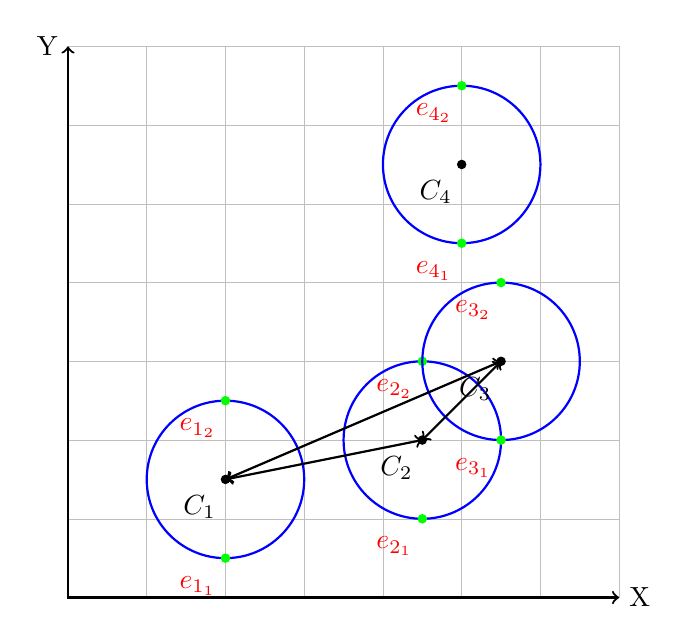
\begin{tikzpicture}[scale=1]
      % grid
      \draw[very thin,color=lightgray] (0,0) grid (7,7);
      \draw [<->,thick] (0,7) node (yaxis) [left] {Y} |- (7,0) node (xaxis) [right] {X};
      
      % Index, x, y, r
      \def\circle[#1,#2,#3,#4] {
    	% The middlepoint
    	\coordinate (C#1) at (#2,#3);
    	
    	
    	% The point
        \draw[fill,color=black] (C#1) circle (1.5pt) node[left, yshift=-10pt, color=black] {$C_#1$};
        
        % The circle
        \draw[thick,color=blue] (C#1) circle (#4);		
        
        % The eventpoints
        \coordinate (E#1_1) at (#2,#3-#4);
        \coordinate (E#1_2) at (#2,#3+#4);
    	
        \draw[fill, color=green] (E#1_1) circle (1.5pt) node[left, yshift=-10pt, color=red] {$e_{#1_1}$};
        \draw[fill, color=green] (E#1_2) circle (1.5pt) node[left, yshift=-10pt, color=red] {$e_{#1_2}$};
      }
      
      \circle[1,2,1.5,1]
      \circle[2,4.5,2,1]    
      \circle[3,5.5,3,1]
      \circle[4,5,5.5,1]
      

      \draw[thick,<->] (C1) -- (C2);
      \draw[thick,<->] (C1) -- (C3);
      \draw[thick,<->] (C2) -- (C3);


      
    \end{tikzpicture}
  }
  \label{fig:voorbeeld_2}
  \caption{Nagekeken cirkels bij algoritme 2}
\end{figure}
\begin{figure}[hbpt]
  \centering
    \begin{tikzpicture}[scale=2]
      % grid
      \draw[very thin,color=lightgray] (0,0) grid (7,7);
      \draw [<->,thick] (0,7) node (yaxis) [left] {Y} |- (7,0) node (xaxis) [right] {X};
      
      \indexedcircle[1,2,1.5,1]
      \indexedcircle[2,4.5,2,1]    
      \indexedcircle[3,5.5,3,1]
      \indexedcircle[4,5,5.5,1]

      \draw[thick,color=blue,arrows={Triangle[scale=1]-Triangle[scale=1]},shorten >=9pt,shorten <=9pt] (C2) -- (C3);

    \end{tikzpicture}
  \label{fig:voorbeeld_23}
  \caption{Nagekeken cirkels bij algoritme 3}
\end{figure}


\section{Resultaten}
%% \todo{grafieken}

\section{Besluit}
%% \todo{besluit}

\listoftodos

\end{document}
